\documentclass[modern]{aastex63}

\usepackage{hyperref}
\usepackage{amsmath}

\let\tablenum\relax
\usepackage{siunitx}

\newcommand{\vdag}{(v)^\dagger}
\newcommand\aastex{AAS\TeX}
\newcommand\latex{La\TeX}

\usepackage{todonotes}

% \received{June 1, 2019}
% \revised{January 10, 2019}
% \accepted{\today}
% \submitjournal{AJ}

\shorttitle{Measuring Wind Speed in DM Space on SCExAO}
\shortauthors{Lucas et al.}

%%%%%%%%%%%%%%%%%%%%%%%%%%%%%%%%%%%%%%%%%%%%%%%%%%%%%%%%%%%%%%%%%%%%%%%%%%%%%%%%
\graphicspath{{./}{figures/}}

\begin{document}

\title{Measuring Wind Speed in DM Space on Subaru Coronagraphic Extreme Adaptive Optics Instrument (SCExAO)}

\author[0000-0001-6341-310X]{Miles Lucas}
\affiliation{Institute for Astronomy, University of Hawai'i \\
2680 Woodlawn Dr, Honolulu, HI 96822, USA}

\author{Michael Bottom}
\affiliation{Institute for Astronomy, University of Hawai'i \\
640 North A‘ohōkū Place Hilo, HI 96720, USA}

\author{Olivier Guyon}
\affiliation{Subaru Telescope, National Astronomical Observatory of Japan \\ 
650 North A‘ohōkū Place, Hilo, HI 96720, USA}
\affiliation{Steward Observatory, The University of Arizona \\
Tucson, AZ 85721, USA}

\author{Vincent Deo}
\affiliation{Subaru Telescope, National Astronomical Observatory of Japan \\ 
650 North A‘ohōkū Place, Hilo, HI 96720, USA}

\begin{abstract}

\end{abstract}

\keywords{}

\section{Introduction}\label{sec:intro}

The last twenty years of astronomy have seen a revolution in planetary science, with thousands of exoplanets discovered around nearby stars. While our understanding of exoplanet demographics has lept forward in recent years, fundamental questions remain. What are the dominant planet formation pathways? How do planetary atmospheres form and evolve? Is there life on other planets?

These questions can only be answered through the spectroscopic characterization of exoplanets over a range of masses and orbital separations from their host stars. While each method of exoplanet detection plays an important role in surveying planets, only the methods of transits and direct imaging allow for the possibility of spectroscopic characterization. Directly imaging exoplanets is versatile- the planet's orbit does not have to transit its host star and the orbital period is less crucial for detection compared to radial velocity, transit, and astrometric methods \citep{2013pss3.book..489W}. The challenge in direct imaging, however, is appropriately separating and nulling the starlight to detect the dim exoplanet signal \citep{2010exop.book..111T}.

The field of direct imaging (or high-contrast imaging) comprises modern instrumentation, observational techniques, and post-processing algorithms to overcome the obstacles in imaging a planet outside our solar system. Adaptive optics (AO) play a critical role in direct imaging by stabilizing the stellar point-spread function (PSF), enabling modern coronagraphs to attenuate the stellar signal \citep{2005ApJ...629..592G}. AO systems consist of a wavefront sensor, deformable mirror, and a real-time controller. The controller takes the images from the wavefront sensor and calculates the deformable mirror commands. This loop needs to run at kHz speeds to enable high-contrast imaging \citep{2018ARA&A..56..315G}.

% Typically, the AO system is ``upstream'' of the science instrument, which means that any wavefront errors ``downstream'' of the wavefront sensor cannot be corrected (e.g., a polishing defect). These wavefront errors are referred to as non-common path aberrations. The aberrations accumulate in the focal plane as quasi-static speckles, which are aberrations of the true PSF \citep{2018ARA&A..56..315G}. The speckles have structure, but it is variable due to slow-changing effects such as thermal gradients. This variability leads to their quasi-static nature.

AO systems are constrained by engineering and runtime factors such as the density of deformable mirror segments, and the speed of the real-time control. These factors limit how well an AO system can correct a wavefront. For ground-based telescopes these limits are significant due to high-speed atmospheric turbulence variation, which evolves faster than the AO system can correct, leading to residual wavefront errors \citep{Soummer_2007}. These errors manifest in fast speckles with coherence times $\sim$0.01s \citep{2018ARA&A..56..315G}, which is much less than a typical science integration ($\sim$10-100s). This causes the speckles to average out over an integration and form a halo with exponentially decreasing brightness from its center. The quasi-static speckles and halo are hard to distinguish from astrophysical signals, limiting our sensitivity to exoplanets (see \autoref{fig:wdh}).

\begin{figure}
    \centering
    % \epsscale{0.7}
    \plotone{wdh}
    \caption{Coronagraphic focal-plane images showing the wind-driven halo effect. The left figure is a simulated model of the SPHERE-IRDIS instrument with a wind-driven halo. The right figure is an H2-band exposure from SPHERE-IRDIS. The circled regions in the right figure are known optical artifacts. The existence of the wind-driven halo greatly compromises the sensitivity for detecting exoplanets in high-contrast imaging. Adapted from \cite{2020AA...638A..98C}.}
    \label{fig:wdh}
\end{figure}
A na\"ive solution to overcome the time-delay would be to run the AO loop at a faster rate, but there is a speed limit due to photon noise on the wavefront sensor when the integration time is too short. For example, on the Subaru telescope with its \SI{8.2}{\meter} aperture, a magnitude 8 star produces approximately \SI{6.9e4}{\photon\per\second} in H-band divided across $\sim$\num{7200} subapertures in the wavefront sensor, which means at \SI{2}{\kilo\hertz} loop rate only 8 photons arrive in each subaperture of each frame. This relationship between loop rate and photon noise is particularly challenging for traditional integrator control laws (the math that determines the deformable mirror commands given the wavefront sensor measurement). These laws use an average of the previous few wavefront measurements to help attenuate the effects of photon noise. This time-averaging, though, exacerbates the time-delay problem and must be carefully balanced for each target. Besides, there will always be the finite time delay of communications and computations within the control system along with mechanical restrictions from the deformable mirror(s). This means there is a fundamental limit to improving performance of wind-driven effects using traditional AO control laws.

\subsection{Predictive wavefront control}\label{sec:pwfc}

Predictive wavefront control improves on traditional AO control laws by \textit{predicting} the future wavefront errors. Predicting the future wavefront would allow extreme AO systems to avoid the time-lag error which creates the wind-driven halo in the focal plane images \citep{2018ARA&A..56..315G}. By forming this prediction off an ensemble of frames in the past, there is also the benefit of reduced photon noise, which means predictive control can enable imaging of fainter targets, too. This is the formulation behind the \textit{Empirical Orthogonal Functions} (EOF; \citealp{guyon_adaptive_2017}) predictive wavefront control law, which uses a linear combination of previous wavefront measurements (which have been projected onto an orthogonal subspace) to predict the future wavefront. Using a linear control law is theoretically well-suited to counteract the effects of wind in the atmosphere, since we believe wind is comprised of a linear combination of flows with constant direction and speed (the \textit{frozen-flow hypothesis}). \citet{guyon_adaptive_2017} reports an expected $\sim$100 times improvement in root-mean-square (RMS) wavefront error using EOF, which leads to $\sim$3 orders of magnitude improved contrast for detecting faint exoplanets. On-sky performance, however, is only a factor of a few improved and in certain cases degenerate non-linear effects overwhelm the algorithm.

\begin{figure}
    \centering
    \epsscale{0.8}
    \plotone{eof-performance}
    \caption{Demonstration of predictive control for high-contrast imaging. The following panels show simulated focal-plane PSF: (a) raw PSF contrast (scale divided by the maximum value), (b) contrast with coronagraphic corrections; here the fast-evolving speckle halo is clear, and (c) contrast with predictive control and coronagraphic corrections. Imaging a Jupiter analogue requires contrast of $\sim10^{-8}$ and for an Earth analogue in reflected light is $\sim10^{-10}$, for reference.}
    \label{fig:eof-perf}
\end{figure}

The shortcoming of predictive control on-sky is an active topic of adaptive optics research \citep{2018ARA&A..56..315G} and is paramount to the success of large-aperture ($>$\SI{10}{\meter}) telescopes for exoplanet imaging. The Thirty Meter Telescope's Planetary Science Imager (PSI) require predictive control to attenuate the time-lag error by at least an order of magnitude to reach their goals of imaging and taking spectra of rocky exoplanets around M-type stars \citep{2018SPIE10703E..0ZG}. This is a parameter space for exoplanets which has not yet been explored by indirect methods and is well-suited for discovering habitable terrestrial planets. Why do the on-sky tests perform so much worse than the testbed results? Is the frozen-flow hypothesis valid in the regime of extreme AO? What are the relevant time scales for the dynamics driving fast speckles? These questions are key to answer in the coming years in order to push ground-based astronomy further in exoplanet research.

\subsection{Studying wind speed}\label{sec:windspeed}

Wind speed is important to study in order to improve current predictive control methods. Alluded to in \autoref{sec:pwfc}, the frozen-flow hypothesis of wind is not guaranteed to be true, and discrepancies may be part of why predictive control does not perform as well on-sky as in theory. In addition, part of the EOF control algorithm requires training a low-rank orthogonal basis to wavefront data. This decomposition is great for filtering sources of wavefront errors like mechanical vibrations since they follow a regular pattern that can be encoded into the subspace. The constant speed and directions of the flows in the frozen-flow hypothesis are likely to be encoded into this subspace, which should improve the prediction of wind-related effects! However, if the flows evolve, by changing direction or speed, this leads to a dramatic decrease in the performance of the predictor. In current applications the EOF predictors are retrained every 30 minutes to alleviate the problems, but a more thorough study of the dynamics of wind speed (how much it changes, and how rapidly) would greatly optimize the application and performance of predictive control. In fact, developing an \textit{online} algorithm that can be run alongside the EOF control law to estimate when to retrain would greatly improve the stability of the wavefront control.

Although it seems obvious to reference atmospheric and meteorological data to determine how wind speed evolves, we instead choose to use telemetry from the AO system itself. While the dynamics of wind evolution are itself an interesting research topic, the concern is with how wind affects the incoming wavefronts. The data-driven approach of using AO telemetry is much more flexible for this scenario than a weather tower, and allows probing the entire atmosphere above the telescope, which would normally require a controlled weather balloon experiment. The rest of this report details how we can use AO telemetry to measure wind speed (\autoref{sec:methods}), including the details of our algorithm (\autoref{sec:algo}) for application on the Subaru Coronagraphic Extreme Adaptive Optics instrument (SCExAO; \citealp{guyon_wavefront_2011}), the verification of the algorithm in simulated and testbed experiments (\autoref{sec:simulated}, \autoref{sec:turbulence}), and the current status of on-sky application of the algorithm (\autoref{sec:onsky}).
\section{Methods}\label{sec:methods}


\begin{deluxetable*}{ccl}
\tabletypesize{\scriptsize}
\tablecaption{Glossary of notation. For constants, the order of magnitude of the constant is given as $\mathcal{O}(\cdot)$, for data structures, the shape (size) of the structure is given.
\label{tbl:definitions}}
\tablehead{\colhead{Symbol} & \colhead{Shape/Size} & \colhead{Description}}
\startdata
\cutinhead{Constants}
$ps_\mathrm{pupil}$ & $\mathcal{O}(10^-1$ \si{\meter\per\pixel}$)$ & pupil platescale \\
$\Delta_\mathrm{px}$ & $\mathcal{O}(1$ \si{\pixel}$)$ & translation between frames \\
$t$ & $\mathcal{O}(10^{-4}$ \si{\second}$)$ & time between frames \\
$f_\mathrm{RTC}$ & $\mathcal{O}(10^3$ \si{\hertz}$)$ & real-time controller loop rate \\
$N$ & $\mathcal{O}(10^2)$ & number of frames to skip (every $N$th frame) \\
$v$ & $\mathcal{O}(10$ \si{\meter\per\second}$)$ & measured wind speed in pupil \\
$\delta v$ & $\mathcal{O}(1$ \si{\meter\per\second}$)$ & wind speed resolution in pupil \\
$v_{\min}$ & $\mathcal{O}(1$ \si{\meter\per\second}$)$ & minimum detectable wind speed in pupil \\
$v_{\max}$ & $\mathcal{O}(10$ \si{\meter\per\second}$)$ & maximum detectable wind speed in pupil \\
$N_t$ & $\mathcal{O}(10^4)$ & number of frames in cube \\
$N_y, N_x$ & (50, 50) & number of pixels per axis per frame \\
\cutinhead{Data Structures}
cube & $(N_t, N_y, N_x)$ & stack of pseudo-open-loop AO telemetry frames \\
mask & $(N_y, N_x)$ & pupil geometry bitmask \\
$\chi$ & $(N_t - N, 2N_y - 1, 2N_x - 1)$ & cross-correlation maps for a given cube \\
\enddata
\end{deluxetable*}

As mentioned in \autoref{sec:windspeed}, we want to use AO telemetry directly for analyzing the dynamics of wind speed. AO telemetry describes any image or derived quantity from the AO system, starting with the wavefront sensor image. Wavefront sensors are located in the \textit{pupil plane}, which means the image is focused on the aperture of of the telescope (see \autoref{fig:pupil}). 

Most modern wavefront sensors (including the pyramid wavefront sensor on SCExAO) operate in ``closed-loop'' mode, which means the deformable mirror is upstream from the wavefront sensor. This means the wavefront sensor is measuring wavefront error \textit{residuals}; effectively the data has already been filtered of as much of the incident wavefront errors as possible. Since we are uniquely concerned with measuring these errors, we opt for using the pseudo-open-loop reconstruction, which emulates an ``open-loop'' AO system (where the wavefront sensor is upstream from the deformable mirror). This means the images are as close to the incident wavefront as possible, correcting for the temporal and spatial filtering imparted by the AO system. SCExAO has an additional complexity to consider: the Subaru telescope has another AO system (AO188; \citealp{2010SPIE.7736E..0NH}) that operates in addition to SCExAO. This means even in the pseudo-open-loop reconstruction SCExAO is seeing the residual wavefront from AO188.

During an observation, as light passes through Earth's atmosphere atmospheric cells reflect and refract the light, causing the amplitude and phase of the wavefront to become incoherent. The pseudo-open-loop reconstruction measures this wavefront in the column of space projected onto the telescope pupil. As wind moves the atmospheric cells in flows the corresponding wavefront errors will translate across the pupil. An example of this motion is shown in \autoref{fig:motion}.

\begin{figure}
    \centering
    \epsscale{0.8}
    \plotone{ao-column}
    \caption{An illustration of the lightpath from a faraway star as seen from the pupil plane of a ground-based telescope. The light enters Earth's atmosphere and will refract through the various atmospheric cells in the column of air above the telescope pupil. Wind can move these cells over time. This column appears projected in the pupil plane, as shown by the image on the right.}
    \label{fig:pupil}
\end{figure}


\begin{figure}
    \centering
    \epsscale{1}
    \plotone{motion}
    \caption{An example of the apparent motion wind is expected to have on wavefront errors in the pupil plane. Here a ``blob'' of wavefront errors, which corresponds to a particular atmospheric cell in the column of air above the pupil, translates about 7 pixels between 400 frames, which corresponds to a wind speed of $\sim$\SI{6}{\meter\per\second} according to the SCExAO loop speed and pupil geometry.}
    \label{fig:motion}
\end{figure}

So, if we can consistently measure the offset between frames we can derive the wind speed. Before addressing how we measure the offsets between frames, let's discuss how we calculate the wind speed from pixel offsets. The SCExAO pupil is an image of the Subaru primary mirror, which is \SI{8.2}{\meter} in diameter. The pupil-plane images we use span this distance with $\sim$48 pixels, so the pupil platescale is approximately \SI{0.17}{\meter\per\pixel}. If there is precise timing information for each frame, we can use that to determine the time delay between frames-
\begin{equation}
    v = \Delta_\mathrm{px} \cdot \frac{ps_\mathrm{pupil}}{t}
\end{equation}
where $\Delta_\mathrm{px}$ is the offset measured in pixels, $ps_\mathrm{pupil}$ is the pupil platescale, and $t$ is the time between frames. We can also use the real-time controller loop rate $f_\mathrm{RTC}$ (e.g., \SI{2}{\kilo\hertz}) to find the average time between $N$ frames-
\begin{equation}
    v = \Delta_\mathrm{px} \cdot \frac{ps_\mathrm{pupil} \cdot f_\mathrm{RTC}}{N}
    \label{eqn:quantity}
\end{equation}

\subsection{Measuring offsets in images}\label{sec:algo}

The previous section derived a formula for wind speed above the telescope pupil but glossed over how to actually measure the offset (or translation) between frames. One of the obstacles to overcome in our data is the effect of the pupil geometry; the pupil shape is effectively a mask. Already this has an effect on our algorithm for deriving wind speeds: if we are measuring offsets between frames sufficiently far apart in time, it is possible that a blob has moved entirely across the pupil, which would be impossible to measure, giving us a maximum measurable wind speed for a given time step (or, equivalently, for the number of frames).
\begin{equation}
    v_{\max} = \frac{8.2\mathrm{ m} \cdot f_\mathrm{RTC}}{N}
    \label{eqn:max}
\end{equation}

One measure for determining how similar two images are is their cross-correlation \citep{1997ApOpt..36.8352F}.
\begin{equation}
    \chi_{i} = \sum_{j}{f_{i}g_{j}}
    \label{eqn:crosscorr}
\end{equation}
where $\chi$ is the cross-correlation map, and $f$ and $g$ are the images in question. The index of the maximum value of $\chi$ corresponds to the amount of translation between $f$ and $g$. 

As mentioned previously, the pupil geometry acts like a mask for our images, which needs to be addressed when using the cross-correlation for measuring offsets. Imagine, for any given frame, there will always be zero signal outside of the pupil, which means that two frames will have extremely high measures of similarity. Since the signal-to-noise ratio (S/N) of these regions is effectively infinite, we want to mask these regions out and let the signal from \textit{within} the pupil drive our cross-correlation. \citet{2012ITIP...21.2706P} derives an efficient cross-correlation algorithm using a bitmask for the two images. We use the implementation from \verb|scikit-image| \citep{2014arXiv1407.6245V} in conjunction with the pupil geometry bitmask stored on the SCExAO control computer.

One consequence of using our masked cross-correlation algorithm is that we can't measure offsets less than half-pixel between frames. The discrete pixels in our images ``bin'' the cross correlation map and any offset less than \SI{0.5}{\pixel} gets binned to \SI{0}{\pixel}. This gives us a natural minimum detectable wind speed
\begin{equation}
    v_{\min} = 0.5\mathrm{ px}\cdot\frac{ps_\mathrm{pupil} \cdot f_\mathrm{RTC}}{N}
    \label{eqn:min}
\end{equation}
In addition, we derive a finite resolution (the bin size) for the wind speed
\begin{equation}
    \delta v = 1\mathrm{ px} \cdot\frac{ps_\mathrm{pupil} \cdot f_\mathrm{RTC}}{N}
    \label{eqn:resolution}
\end{equation}

Combining \autoref{eqn:max} and \autoref{eqn:min} helps guide our choice of how far apart we should measure frames for offsets. SCExAO typically operates at \SI{2}{\kilo\hertz}, and we expect wind speeds to be between $\sim$\SIrange{0}{60}{\meter\per\second}. Using every 300th frame ($N=300$) would give a minimum detectable speed of \SI{0.6}{\meter\per\second} and maximum detectable speed of \SI{55}{\meter\per\second}. In practice, we found that using every 400th frame ($N=400$) worked well.

As mentioned with regards to the pupil geometry, any static signal between images will dominate the cross-correlation compared to any moving signal. To help alleviate this, we perform multiple pre-processing steps to our data before measuring the masked cross-correlation. The SCExAO control computer can save \textit{pseudo-open-loop} frames as a cube of images, with $\mathcal{O}(10^4)$ frames per cube (which only corresponds to tens of seconds due to high loop rate). Pseudo-open-loop frames are used because they represent the highest S/N of wavefront errors in the pupil plane and have already been processed and filtered by the SCExAO real-time controller to remove systematics (like the deformable mirror flat frames).

Our first pre-processing step is to subtract out a median frame from the data cube, which helps remove static structure that may corrupt the cross-correlation. Without this step, we find that even the most trivial of datasets cannot effectively retrieve offsets between frames; removing static signal is paramount to having a bias-free cross-correlation. Another step we take to remove further static signal is filtering low-order Zernike modes out of our data. We do this because we expect the translational signal to be high spatial frequency, and we need to remove as much non-translational signal as possible. Another spatial filter we apply is a Gaussian high-pass filter. We accomplish this by convolving a Gaussian with \SI{5}{\pixel} spatial standard deviation and 1 frame temporal standard deviation to our data, and then subtracting this output from the cube. We found this chain of pre-processing is sufficient for testbed data and is a promising start for on-sky data, which will be discussed in \autoref{sec:onsky}. The full algorithm is listed in Algorithm~\autoref{alg:windspeed}.

\begin{algorithm}
\caption{wind speed measurement}\label{alg:windspeed}
\begin{algorithmic}[0]
\State $\mathbf{cube:}$ pseudo-open-loop full frame data ($N_t$, $N_y$, $N_x$)
\State $\mathbf{mask:}$ pupil bitmask ($N_y$, $N_x$)
\Procedure{WindSpeed}{cube, $N$, $f$, $n_Z$=7, stds=(1, 5, 5)}
    \State tmp $\gets$ cube - project\_zernike(cube, $n_Z$) \Comment{Filter out low-order Zernike modes}
    \State tmp $\gets$ tmp - median(tmp) \Comment{Subtract median frame}
    \State tmp $\gets$ tmp - gaussian\_filter(tmp, stds) \Comment{Gaussian high-pass filter}
    \For{$k$ in 1..($N_t-N$)} \Comment{For each frame in cube}
        \State previous $\gets$ tmp[$k$]
        \State current $\gets$ tmp[$k+N$]
        \State $\chi$[$k$] = masked\_cross\_correlate(current, previous, mask)
        \State idx $\gets$ argmax($\chi$[$k$])
        \State offset $\gets$ idx - ($N_y$, $N_x$) + 1 \Comment{Have to correct for geometry of cross-correlation}
        \State speed[$k$] $\gets$ offset $\cdot ps_\mathrm{pupil} \cdot f / N$
    \EndFor
    \State $\mathbf{return}$ $\chi$, speed
\EndProcedure
\end{algorithmic}
\end{algorithm}

\section{Results}\label{sec:results}
\subsection{Simulated turbulence}\label{sec:simulated}

To validate our algorithm, first we simulate atmospheric turbulence and try and directly measure wind speed without any interaction with the telescope optics. To do this, we emulate the procedure from \citet[sec.~4.1]{guyon_adaptive_2017}, which generates a phase screen with \SI{2}{\micro\meter} RMS wavefront error, which corresponds to a Fried parameter of $r_0=$\SI{20}{\centi\meter}, matching typical good seeing on Mauna Kea. Seven atmospheric layers are simulated using Von Karman statistics and summed together using the frozen-flow hypothesis \citep[see][tbl.~1]{guyon_adaptive_2017}. We simulated three different wind speeds, 3, 6, and \SI{10}{\meter\per\second}. For each simulation, we generate a cube with \num{10000} frames and measure offsets using Algorithm~\autoref{alg:windspeed}.

\begin{figure}
    \centering
    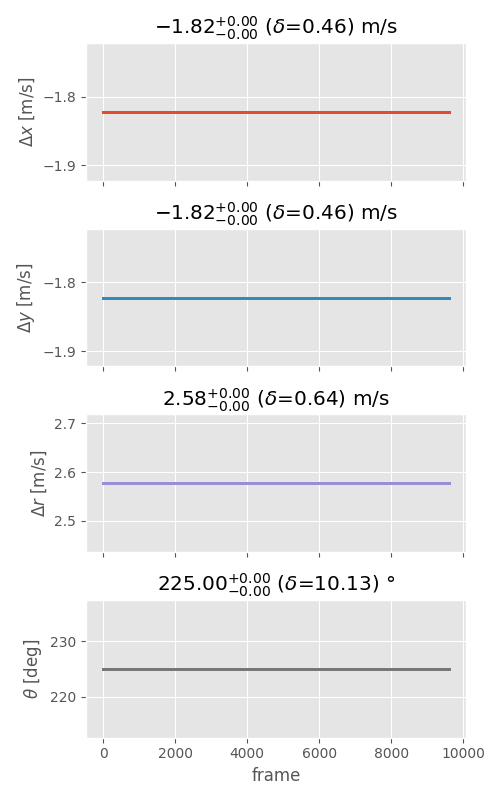
\includegraphics[width=0.32\textwidth]{chains_3ms}
    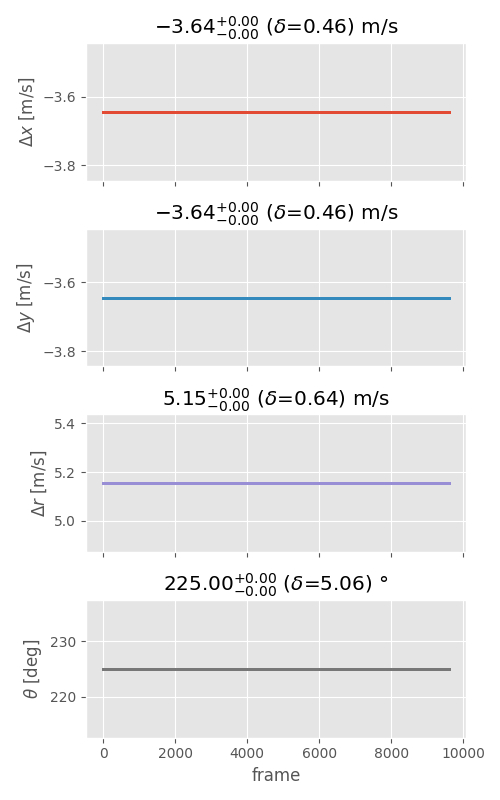
\includegraphics[width=0.32\textwidth]{chains_6ms}
    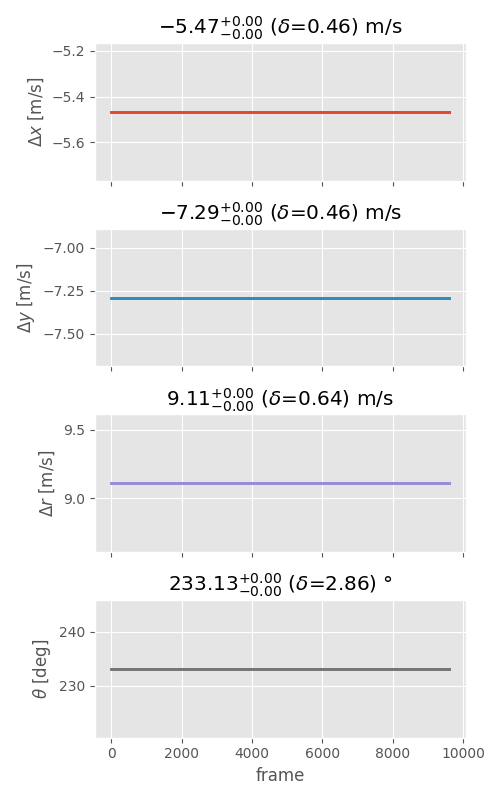
\includegraphics[width=0.32\textwidth]{chains_10ms}
    \caption{Offsets measured from simulated wavefront data. Printed above each chain is the median value, the spread of the inner quartile, and the resolution of the measurement. The offsets in $x$ and $y$ are the first two rows (red, blue). The vector magnitude $r$ and direction $\theta$ are the last two rows (purple, gray). The first column has \SI{3}{\meter\per\second} simulated wind speed. The second column has \SI{6}{\meter\per\second} simulated wind speed, and the last column has \SI{10}{\meter\per\second} simulated wind speed.}
    \label{fig:simulated}
\end{figure}

In \autoref{fig:simulated}, we can see the offsets measured by our algorithm on the simulated turbulence data. The magnitude of the wind speed for each cube (third row, purple) is very close to the true value. Any discrepancies here can be explained by slight differences in calibration (like the pupil platescale). The direction of the translation matches the visual flow in the input data.

\subsection{Simulated turbulence on the SCExAO testbed}\label{sec:turbulence}

The previous experiment does not include any details of the AO system or telescope optics. To address this, we further validate our algorithm on the SCExAO testbed \citep{guyon_wavefront_2011}. The testbed includes internal light sources which allow running the AO loop and taking data during off-hours. We use the testbed with the internal light source as a baseline for our next experiment. In this test, we take the simulated turbulence from \autoref{sec:turbulence} and manually inject the wavefront errors onto the deformable mirror. Once we have the AO loop running and the have adjusted the gain after injecting the wavefront errors, we again save a cube of 10,000 frames for analysis with Algorithm~\autoref{alg:windspeed}.

\begin{figure}
    \centering
    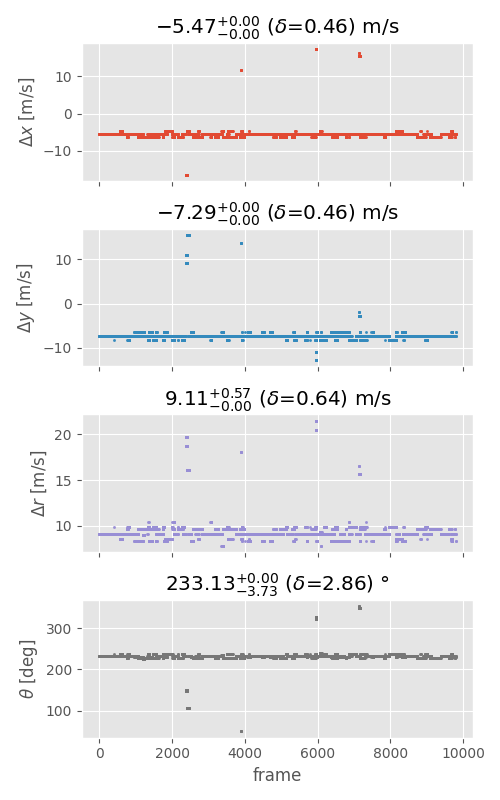
\includegraphics[width=0.35\textwidth]{chains_testbed}
    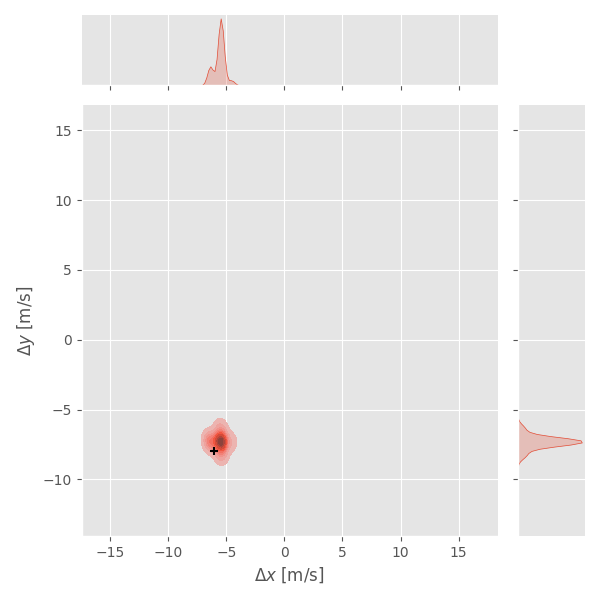
\includegraphics[width=0.5\textwidth]{radial_testbed}
    \caption{Offsets measured from injected turbulence with \SI{10}{\meter\per\second} wind speed on the SCExAO testbed using an internal light source. The left plots show chains for the offsets, while the right plot shows the kernel density estimate (KDE) of the measurements. Printed above each chain is the median value, the spread of the inner quartile, and the resolution of the measurement. The true value of \SI{10}{\meter\per\second} is marked by a cross in the 2-D KDE plot.}
    \label{fig:testbed}
\end{figure}

In \autoref{fig:testbed} we see that the \SI{10}{\meter\per\second} wind speed is recovered well, even with the added complexities of the SCExAO system. We are satisfied with the performance of the algorithm using simulated data on the testbed.

\subsection{On-sky SCExAO data}\label{sec:onsky}

In order to study the dynamics of wind speed, we need to apply our algorithm on-sky. The SCExAO team keep an archive of previous observations with saved AO telemetry. While not every observation includes the pseudo-open-loop telemetry we need for our algorithm, there are many half-nights with hours of the telemetry we need saved. Ideally, we could take the data cubes from each of these nights, apply our algorithm to them, and create a chain of wind speed measurements over many hours. These chains could then be analyzed for dynamic changes in the wind, such as the time scale for changing wind directions. These are the results we want to analyze for improving predictive control methods.

As a start, we found AO data that has a visible flow which may correspond to wind in the atmosphere. By visual inspection, the flow appears to have $\sim$\SI{3}{\pixel} motion over 200 frames at $\sim$ \SI{90}{\degree}. This data was taken while the AO loop was running at \SI{3.5}{\kilo\hertz}, so the corresponding wind speed is $\sim$\SI{9}{\meter\per\second}. Visibly this data suffers from far more systematics than the testbed data with regards to our algorithm. For example, on-sky data has a pronounced tip-tilt ``beating'', which is what inspired the modal filtering in Algorithm~\autoref{alg:windspeed}. In addition, the on-sky data is generally much noisier and often suffers from low-wind effect (LWE), which causes the quadrants in the pupil delimited by the secondary support spiders to ``petal" out. Spurious, noisy correlations dominate the outputs, shown in \autoref{fig:onsky}.

\begin{figure}
    \centering
    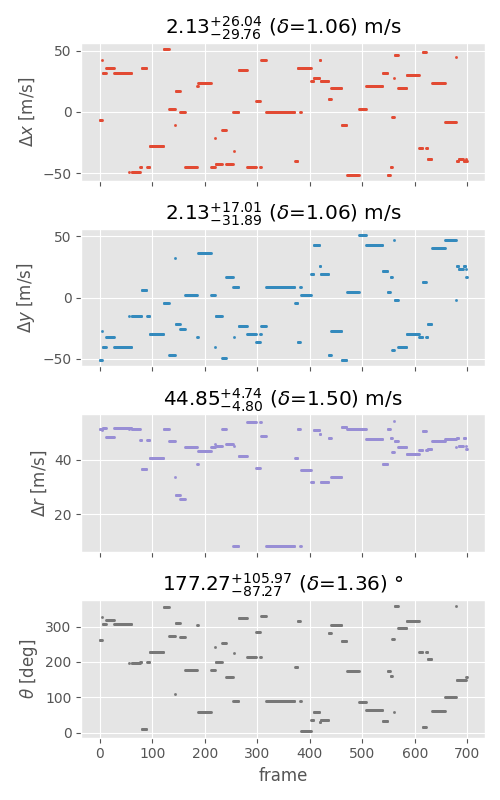
\includegraphics[width=0.35\textwidth]{chains_onsky}
    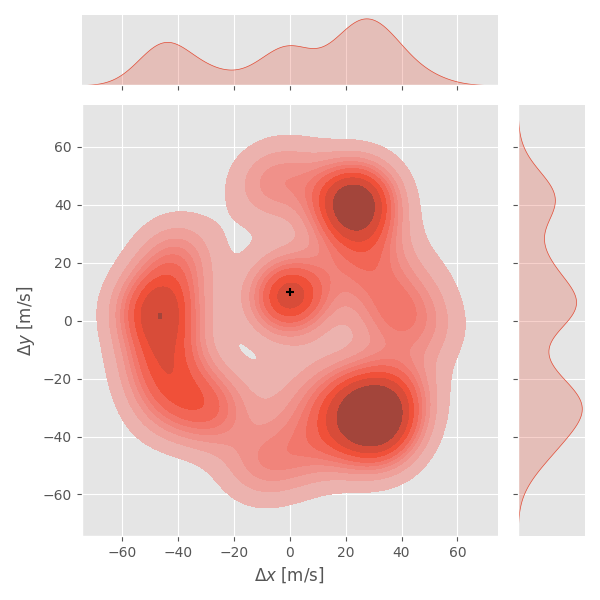
\includegraphics[width=0.5\textwidth]{radial_onsky}
    \caption{Offsets measured from on-sky SCExAO data. The left plots show chains for the offsets, while the right plot shows the 2-D marginal kernel density estimate (KDE) of the $x$ and $y$ measurements. Printed above each chain is the median value, the spread of the inner quartile, and the resolution of the measurement. The marginal KDE is cropped to only show detectable values according to \autoref{eqn:max}. The apparent motion between frames is marked with a black cross in the 2-D KDE plot.}
    \label{fig:onsky}
\end{figure}

The value we expected to retrieve is seen in the marginal distribution of \autoref{fig:onsky} ($\sim$\SI{9}{\meter\per\second} at \SI{90}{\degree}), which means our algorithm is working \textit{sometimes}. It is notable that the spurious offset measurements tend to occur in a ring close to the maximum detectable wind speed, which is even more pronounced if we do less aggressive modal and high-pass filtering.

\section{Conclusions} \label{sec:conclusions}


\software{}

\bibliography{references}{}
\bibliographystyle{aasjournal}

\appendix

\end{document}
